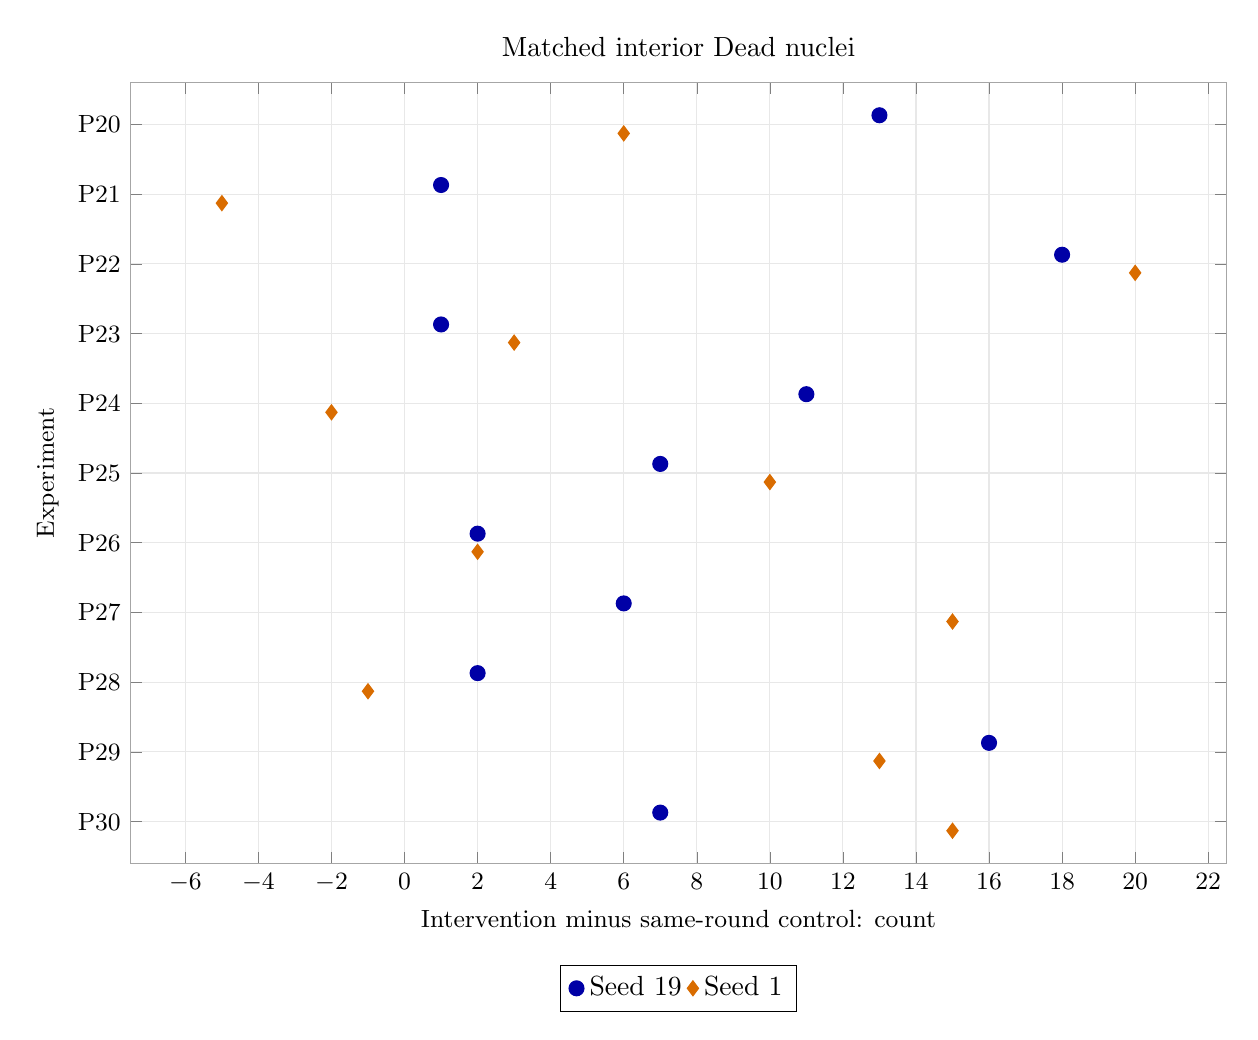
\begin{tikzpicture}
\begin{axis}[width=15.5cm,height=11.5cm,xlabel={Intervention minus same-round control: count},ylabel={Experiment},title={Matched interior Dead nuclei},ytick={0,1,2,3,4,5,6,7,8,9,10},yticklabels={P20,P21,P22,P23,P24,P25,P26,P27,P28,P29,P30},ymin=-.6,ymax=10.6,y dir=reverse,grid=major,grid style={gray!18},legend style={at={(.5,-.13)},anchor=north,legend columns=2},axis line style={gray!70},tick label style={font=\small},label style={font=\small},title style={font=\normalsize}]
\addplot[only marks,mark=*,mark size=2.7pt,color=blue!65!black] coordinates {(13,-0.13) (1,0.87) (18,1.87) (1,2.87) (11,3.87) (7,4.87) (2,5.87) (6,6.87) (2,7.87) (16,8.87) (7,9.87)};
\addlegendentry{Seed 19}
\addplot[only marks,mark=diamond*,mark size=2.7pt,color=orange!85!black] coordinates {(6,0.13) (-5,1.13) (20,2.13) (3,3.13) (-2,4.13) (10,5.13) (2,6.13) (15,7.13) (-1,8.13) (13,9.13) (15,10.13)};
\addlegendentry{Seed 1}
\end{axis}
\end{tikzpicture}
